\chapter{Neuronale Netzwerke}

Unter einem neuronalen Netzwerk versteht man ein System
aus Neuronen. Diese sind schichtweise organisiert wobei
jedes Neuron einer Schicht jeweils zu allen Neuronen der
direkt anliegenden Schichten verbunden ist.
Abbildung \ref{fig:Neuronales Netzwerk} zeigt beispielhaft ein
neuronales Netzwerk aus 19 Neuronen mit insgesamt 5 Schichten.
\bigskip

\begin{figure}[h]
    \begin{center}
        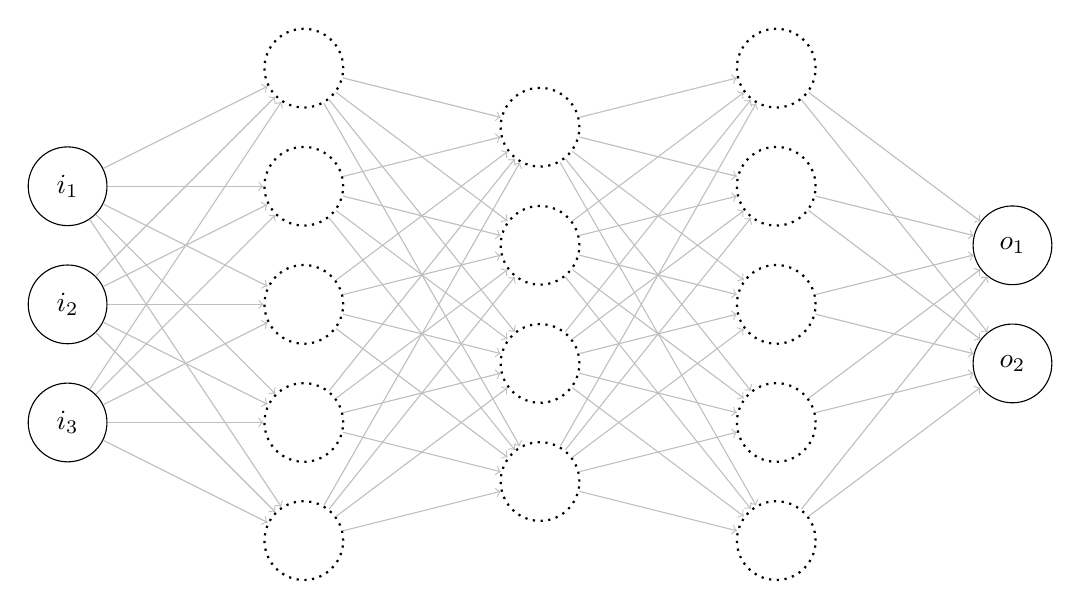
\begin{tikzpicture}[y=-1.5cm,x=3cm]
            \tikzset{
                netnode/.style={circle,draw=black,minimum size=1cm},
                hidden/.style={dotted,thick}
            }
            \node[netnode] (i1) at (0,0) {$i_1$};
            \node[netnode] (i2) at (0,1) {$i_2$};
            \node[netnode] (i3) at (0,2) {$i_3$};

            \node[netnode,hidden] (l11) at (1,-1) {};
            \node[netnode,hidden] (l12) at (1,0) {};
            \node[netnode,hidden] (l13) at (1,1) {};
            \node[netnode,hidden] (l14) at (1,2) {};
            \node[netnode,hidden] (l15) at (1,3) {};

            \node[netnode,hidden] (l21) at (2,-0.5) {};
            \node[netnode,hidden] (l22) at (2,0.5) {};
            \node[netnode,hidden] (l23) at (2,1.5) {};
            \node[netnode,hidden] (l24) at (2,2.5) {};

            \node[netnode,hidden] (l31) at (3,-1) {};
            \node[netnode,hidden] (l32) at (3,0) {};
            \node[netnode,hidden] (l33) at (3,1) {};
            \node[netnode,hidden] (l34) at (3,2) {};
            \node[netnode,hidden] (l35) at (3,3) {};

            \node[netnode] (o1) at (4,0.5) {$o_1$};
            \node[netnode] (o2) at (4,1.5) {$o_2$};

            \foreach \i in {1,2,3}{
                    \foreach \j in {1,...,5}{
                            \draw[->,black!25] (i\i) -- (l1\j);
                        }
                }
            \foreach \i in {1,...,5}{
                    \foreach \j in {1,...,4}{
                            \draw[->,black!25] (l1\i) -- (l2\j);
                        }
                }
            \foreach \i in {1,...,4}{
                    \foreach \j in {1,...,5}{
                            \draw[->,black!25] (l2\i) -- (l3\j);
                        }
                }
            \foreach \i in {1,...,5}{
                    \foreach \j in {1,2}{
                            \draw[->,black!25] (l3\i) -- (o\j);
                        }
                }
        \end{tikzpicture}
    \end{center}
    \caption{Neuronales Netzwerk}
    \label{fig:Neuronales Netzwerk}
\end{figure}

\section{Neuronen}

Unter einem Neuron versteht sich bei neuronalen Netzen lediglich ein Knoten,
in dem üblicherweise ein 32-bit großer Wert hinterlegt ist. Häufig kommen hier
Gleitkommazahlen zwischen -1.0 und 1.0 zum Einsatz, da sich dieser Wertebereich
besonders gut zum Rechnen eignet und Eigenschaften bezüglich der
Multiplikation besitzt, die eine Wertexplosion verhindern.
Die Werte aller Neuronen, mit Ausnahme derer in der Eingabeschicht, setzen sich
jeweils aus den Werten aller Neuronen der direkt davor liegenden Schicht zusammen.
Das genaue Vorgehen bei der Wertermittlung hängt jeweils vom Netzwerk
und den dort verwendeten Aktivierungsfunktionen ab.

\section{Schichten und Kanten}

In einem neuronalen Netzwerk ist jedes Neuron einer Schicht mit allen Neuronen
der jeweiligen davor liegenden und danach liegenden Schicht über Kanten verbunden.
Neuronale Netzwerke sind unidirektionale Graphen, demnach fließen Informationen
über Schichten (und folglich Kanten) nur in eine Richtung.

Allen Kanten wird initial eine Gewichtung zugewiesen, welche erneut
netzwerkabgängig generiert werden oder durch zuvor angelernte Daten bestimmt
werden. Beim Trainieren des Netzwerks werden diese bei jeder Lerniteration
(auch \emph{Epoch} genannt) justiert, während sie beim Betrieb für gewöhnlich
keine Änderungen mehr erfahren.
Die Genauigkeit eines Netzwerks wird überwiegend durch diese Gewichte bestimmt,
daher ist das Ziel beim Trainieren eines Netzes die Optimierung jener.

Kantengewichte wirken sich maßgeblich auf die Wertberechnung von Neuronen aus.
Diese wird in zwei Schritten ausgeführt. Im ersten Schritt wird aus den
Kantengewichten ($e_{i}$) aller eingehenden Kanten und den Werten der darüber
verbundenen Neuronen ($v_{i}$) der Wert nach Formel (2.1) gebildet.

\begin{align}
    v=\sum_{i=1}^{n}(e_{i} * v_{i})
\end{align}

\section{Aktivierungsfunktionen}

Im zweiten Schritt wird der zuvor errechnete Wert durch eine weitere Funktion
modifiziert. Sogenannte \emph{Aktivierungsfunktionen} können beliebig gewählt
werden, müssen jedoch offensichtlich alle möglichen Eingaben auf einen Wert
abbilden können. Die verwendete Aktivierungsfunktion kann je nach
Schicht variieren. Einmal gewählt, ist diese jedoch für die jeweilige Schicht
im Netzwerk fest.

Im Folgenden sind sind häufig verwendete Aktivierungsfunktionen und ihre Formeln
abgebildet.

\begin{figure}[H]
    \begin{minipage}{0.45\textwidth}
        \begin{center}
            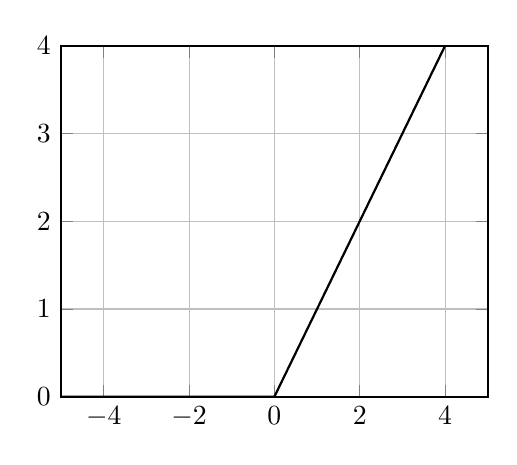
\begin{tikzpicture}
                \begin{axis}[width=7cm,xmin=-5,xmax=5,ymin=0,ymax=4,thick,grid=both]
                    \addplot[] {max(x,0))};
                \end{axis}
            \end{tikzpicture}
        \end{center}
        \caption{ReLU}
    \end{minipage}\hfill
    \begin{minipage}{0.45\textwidth}
        \begin{center}
            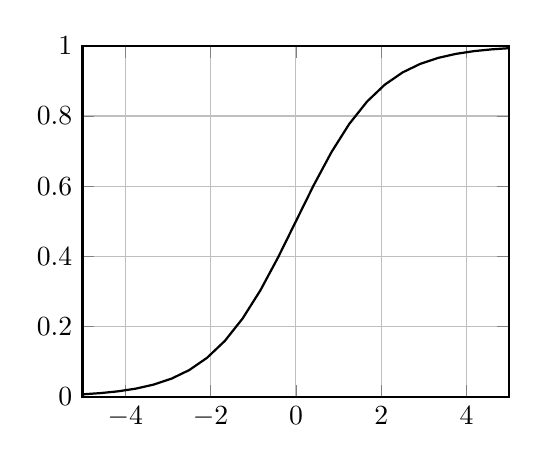
\begin{tikzpicture}
                \begin{axis}[width=7cm,xmin=-5,xmax=5,ymin=0,ymax=1,thick,grid=both]
                    \addplot[] {1/(1+exp(-x))};
                \end{axis}
            \end{tikzpicture}
        \end{center}
        \caption{Sigmoid}
    \end{minipage}
\end{figure}
%
\begin{figure}[H]
    \begin{minipage}{0.45\textwidth}
        \begin{center}
            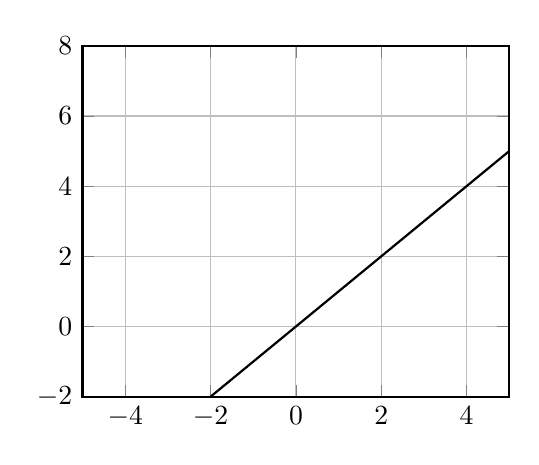
\begin{tikzpicture}
                \begin{axis}[width=7cm,xmin=-5,xmax=5,ymin=-2,ymax=8,thick,grid=both]
                    \addplot[] {x};
                \end{axis}
            \end{tikzpicture}
        \end{center}
        \caption{Softmax}
    \end{minipage}\hfill
    \begin{minipage}{0.45\textwidth}
        \begin{center}
            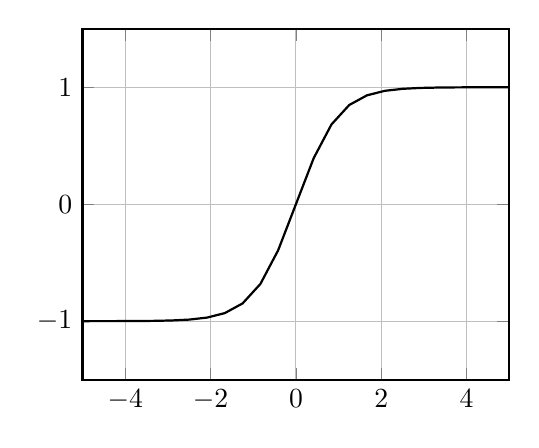
\begin{tikzpicture}
                \begin{axis}[width=7cm,xmin=-5,xmax=5,ymin=-1.5,ymax=1.5,thick,grid=both]
                    \addplot[] {(exp(x)-exp(-x)) / (exp(x)+exp(-x))};
                \end{axis}
            \end{tikzpicture}
        \end{center}
        \caption{tanh}
    \end{minipage}
\end{figure}

Die beiden erläuterten Berechnungsschritte werden schichtweise in Richtung des
Datenflusses des Netzwerks für alle Neuronen durchgeführt.

\section{Training}

\section{Backpropagation (?)}

